\subsection{Reactor Pattern}
\label{section:Reactor Pattern}

Das Reactor Pattern ist ein Design Pattern bei dem asynchrone auftretende Events, synchron abgearbeitet werden können. Dabei werden eingehende Nachrichten/Events von mehreren Clients sequentiell abgearbeitet. Durch das Reactor Pattern können nicht blockierende Applikationen entwickelt werden. Da das registrieren und aufrufen von Ereignissen vom Reactor Pattern übernommen wird gibt es eine lose Koppelung zwischen dem Lesen von I/O Operationen und der Applikation. \cite[p. 1]{Sch95}


\subsubsection{Motivation}

Douglas C. Schmidt beschreibt einen Anwendungsfall für das Reactor Pattern, bei dem Logging Informationen in einem Verteilten System an einen zentralen Server gesendet und gespeichert werden. Der Server soll in der Lage sein Logging informationen zu jederzeit speichern zu können und Logging Informationen können auch von mehreren Clients gleichzeitig an den Server gesendet werden. Möchte ein Client eine Verbindung zum Webserver aufbauen, wird der Thread des Webservers so lange blockiert, bis die Verbindung aufgebaut wurde und alle Daten übertragen wurden \cite[p. 1]{Sch95}. Sektion \ref{subsection: i/o speed} vergleicht wie lange I/O Operationen benötigen.

Eine Möglichkeit um mehrere Verbindungen auf einmal zu verarbeiten bietet Multithreading. Laut D. Schmit bringt diese Lösung jedoch folgende Probleme mit sich \cite[p. 2]{Sch95}:

\begin{itemize}
  \item Benötigt ein komplexes concurrency Schema
  \item Auf Single Core Prozessoren kann es zu einer schlechten Performance kommen
  \item Es könnte nicht auf allen Betriebssystemen verfügbar sein.
\end{itemize}

Die Nachteile 2 und 3 können 20 Jahre nach dem erscheinen dieses Papers als hinfällig angesehen werden, da mittlerweile multicore Prozessoren im Consumer Bereich angekommen sind und jedes relevante Betriebssystem Threads unterstützt. Das Problem Nummer 1 mit dem komplexen concurrency Schema bei der Verwendung von Multithreading bleibt bis heute bestehen.

\subsubsection{Funktionsweise}

Das Reactor Pattern implementiert eine Event Loop welche sich um das event demultiplexen und das event handler dispatchen kümmert. Dabei ist der Reactor ein Prozess mit einer endlosen Schleife (= Event Loop) der auf äußerde Ergebnisse reagiert. Um auf Ereignisse von außerhalb reagieren zu können müssen Callback Funktionen definiert werden, welche ausgeführt werden, wenn ein bestimmtes Ereignis eintritt. Dadurch kann eine Applikation auf die Ereignisse reagieren, für welche eine Callback Funktion definiert ist. In der Regel werden Callback Funktionen ausgeführt wenn eine blockierende I/O Operation abgeschlossen ist. Dabei können typische Ereignisse folgende sein \footnote{Die Liste ist angelehnt an folgenden Blog-Post: \url{http://pltconfusion.com/2014/10/20/eventmachine_internals_and_the_reactor_pattern/}}:

\begin{itemize}
  \item Eine Datei wurde von einem Filesystem gelesen
  \item Eine Datebank abfrage wurde gelesen
  \item Ein HTTP Request wurde kompletiert
\end{itemize}

Wie genau die Eventloop einzelne Ereignisse behandelt variiert zwischen den einzelnen Implementierungen. Eine Mögliche Implementierung ist das Ereignis an das Ende einer Queue zu geben und bei jedem durchlauf der Eventloop wird genau ein Ergebnis von der Queue genommen und behandelt. 

\begin{figure}[!htb]
  \centering
  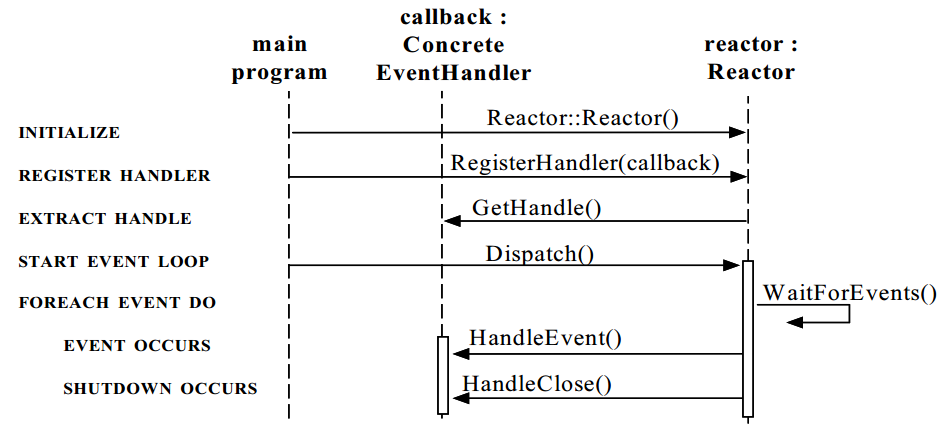
\includegraphics[width=10cm]{images/reactor.png}
  \caption{
    Websocket Data Framing \cite[p. 5]{Sch95}
  }
  \label{figure:WSDataFraming}
\end{figure}








Durch das Reactor Pattern wird eine enge Koppelung zwischen unabhängigen Teilen der Applikation und Applikations abhängigen teilen gelöst. Dadurch werden die Tief liegenden und komplexen Componenten wie das Demultiplexing von Events von der Event Loop übernommen und der Programmierer kann sich auf die eigentliche Applikation konzentrieren. \cite[p. 2]{Sch95}


\subsubsection{Reactor - Design Pattern}

Im folgenden wird das Reactor Design Pattern in der OTM Notation vorgestellt. \footnote[0]{Mehr Informationen zur OTM Notation: \url{http://www.uml.org/}}

(TODO: add image of the design pattern and citation)

\cite[p. 2]{Sch95}

\emph{Reactor}
	Definiert ein Interface um EventHandler Objekte zu registrieren, entfernen und dispatchen. Der Reactor ist Applikationsunabhängig, kann jedoch Applikationsabhängige Ereignisse dispatchen und demultiplexen.

\emph{Event Handler}
	Definiert ein Interface um callback funktionen zu dispatchen.

\emph{ConcreteEventHandler}
	Definiert und Implementiert die Applikationsabhängigen Callback Methoden.

\subsubsection{Funktionsweise}
Event Handler werden beim eintreten eines Events aufgerufen. Diese Events werden über Callback Methoden auf die jeweiligen Betriebssystem I/O Handlern gebunden. Um einen Eventhandler mit dem Reactor zu verbinden muss die Subklasse von Event Handler die Methode \emph{getHandler()} implementieren. Bei der Initialisierung ruft der Reactor die \emph{getHandler()} Methode auf und benutzt diese um auf ein Ereignis zu warten. Der Reactor verwaltet eine Liste mit allen registrieren Event Handler und beim eintreten eines Events löst er das Ereignis aus und ruft die registrierte Callback Funktion auf \cite[p. 5]{Sch95}. (TODO: refactor)

(TODO: what is thread blocking)
(TODO: Add Image)

Ein Beispiel für das Reactor Pattern ist die Kommunikation zwischen einem File System und der Applikation.


\subsubsection{Anwendungsgebiete}

Douglas Schmidt beschreibt in seiner Thesis folgende Anwendungsgebiete für das Reactor Pattern \cite[p. 4]{Sch95}:

\begin{itemize}
  \item Ein oder mehrere Ereignisse können gleichzeitig von unterschiedlichen Clients kommen
  \item Das Blockieren eines Clients oder das Pollen von Requests ist zu ineffizient
  \item Die gesendeten Nachrichten können in relativ kurzer Zeit verarbeitet werden
  \item Wenn unabhängige Teile der Applikation (Event Demultiplexing/Dispatching) von den abhängigen getrennt werden sollen
\end{itemize}

\subsubsection{Zusammenfassung}

Das Reactor Pattern ist ein Designpattern um asynchron auftretende Ereignisse in einen Synchronen Datenfluss zu verwandeln. Dabei verwendet es eine Event-Loop um auf asynchrone Ereignisse zu warten und ruft beim eintreten des Ereignisses die richtige Callback Funktion auf. Durch die Event-Loop kann das Reactor Pattern auf einem einzelnen Thread implementiert werden. Dadurch wird kein komplexes concurrency Schema wie bei Threads benötigt.